\documentclass[12pt,a4paper]{article}
\usepackage[utf8]{inputenc}
\usepackage[T1]{fontenc}
\usepackage[magyar]{babel}
\usepackage{graphicx}
\usepackage{geometry}
\usepackage{fancyhdr}
\usepackage[hidelinks]{hyperref}
\usepackage[numbers]{natbib}
\usepackage{subcaption}

% \geometry{a4paper, margin=35mm, headheight=15mm}
\geometry{paperwidth=305mm, paperheight=297mm, left=35mm, right=130mm, top=35mm, bottom=35mm, headheight=15mm, marginparwidth=120mm}
\setlength{\marginparwidth}{120mm}
\usepackage{marginfix}
\usepackage[colorinlistoftodos]{todonotes}
\usepackage{soul}
\definecolor{vikinote}{RGB}{185,175,240}
\newcommand{\viki}[2][]{\ifx&#1&\par\noindent{\color{violet!70}\Large*}\todo[color=vikinote!50,bordercolor=violet!70,linecolor=violet!80,fancyline]{\textbf{Viki:} #2}\par\else\todo[color=vikinote!50,bordercolor=violet!70,linecolor=violet!80,fancyline]{\textbf{Viki:} #2}\hl{#1}\fi}

\pagestyle{fancy}
\fancyhf{}
\fancyhead[L]{\footnotesize\sc Vesetranszplantációs cserekörök egészértékű programozással}
\fancyhead[R]{\thepage}
\renewcommand{\headrulewidth}{0.4pt}
\renewcommand{\footrulewidth}{0pt}

\begin{document}

%% --------------------------------------------------------
%% Előlap
%% --------------------------------------------------------
\begin{titlepage}
\thispagestyle{empty}
\begin{center}

\includegraphics[height=18mm]{bme_logo_kicsi}

\vspace{2cm}

{\large\sc BSc Önálló Laboratórium Beszámoló}

\vspace{1.5cm}

{\LARGE\bf
Orvosi kritériumoknak megfelelő vesetranszplantációs cserekörök meghatározása egészértékű programozással
}

\vspace{1.5cm}

{\large Szigeti Tibor}

\vspace{1cm}

{\large Tanszéki konzulens: Nemkin Viktória}\\[0.3cm]
% {\large Külső konzulens: Biró Péter}

\vfill

{\sc Budapesti Műszaki és Gazdaságtudományi Egyetem\\
Villamosmérnöki és Informatikai Kar\\
Számítástudományi és Információelméleti Tanszék}

\vspace{0.8cm}

{\large Budapest, \the\year}

\end{center}
\end{titlepage}

%% --------------------------------------------------------
%% Tartalomjegyzék
%% --------------------------------------------------------
\tableofcontents
\newpage

%% --------------------------------------------------------
%% Tartalom
%% --------------------------------------------------------

\section{Bevezetés}
A laboratórium témája a vesetranszplantációs cserekörök meghatározására \viki[próbál]{A téma nem próbál megoldást adni, ez nyelvtanilag hibás. A dolgozat témája vesetranszplantációs cserekörök keresése és te próbálsz megoldást adni. :)} megoldást adni. Ötletének forrása a páneurópai vesecsere program.

\viki{Itt a bevezetésben kellene sokkal többet mesélni arról, hogy mi egyáltalán ez a program és hogyan működik, először még a szakkifejezések használata nélkül, motiválni az olvasót.}

\subsection{Szakkifejezések}
\begin{itemize}
	\item Recipient-donor pair (RDP) - recipiens-donor pár
	
	A modellező gráfban is megjelenített ábrán a csúcspontokat alapvetően két személy alkotja. Egy donor és egy recipiens pár.

	\item Non-directed donors (NDD) / altruistic donors - altruista donor vagy önzetlen donor
	
	Olyan élő donor, aki nem egy konkrét személynek (például rokonnak vagy barátnak), hanem az országos/nemzetközi várólistán szereplő bármely rászoruló számára ajánlja fel a szervét.
\viki{(Javaslat) Ha ennél sokkal több szakkifejezés nem lesz, akkor akár bele is fűzheted a bevezetőbe ezt a két kifejezést. Általában ha egy nagyon rövid fejezeted van, azt inkább érdemes összevonni más fejezetekkel. }
\end{itemize}

\subsection{Modellező gráf}
Két ember egy \viki[pont]{Általában inkább a csúcs kifejezést szoktuk használni, a pontot szerintem akkor, ha valami geometriai kontextus is van.}, ami egy donort és egy recipienst jelent. \viki[A súlyozott, irányított élek a köztük lévő potenciális csere erőssége.]{Ebből nem derül ki, hogy az él melyik irányba mutat illetve az "erőssége" kifejezés ködös. Itt gondolom ennek sok definíciója létezik, de egy egyszerű példa még segítene.}

\begin{tabular}{c c}
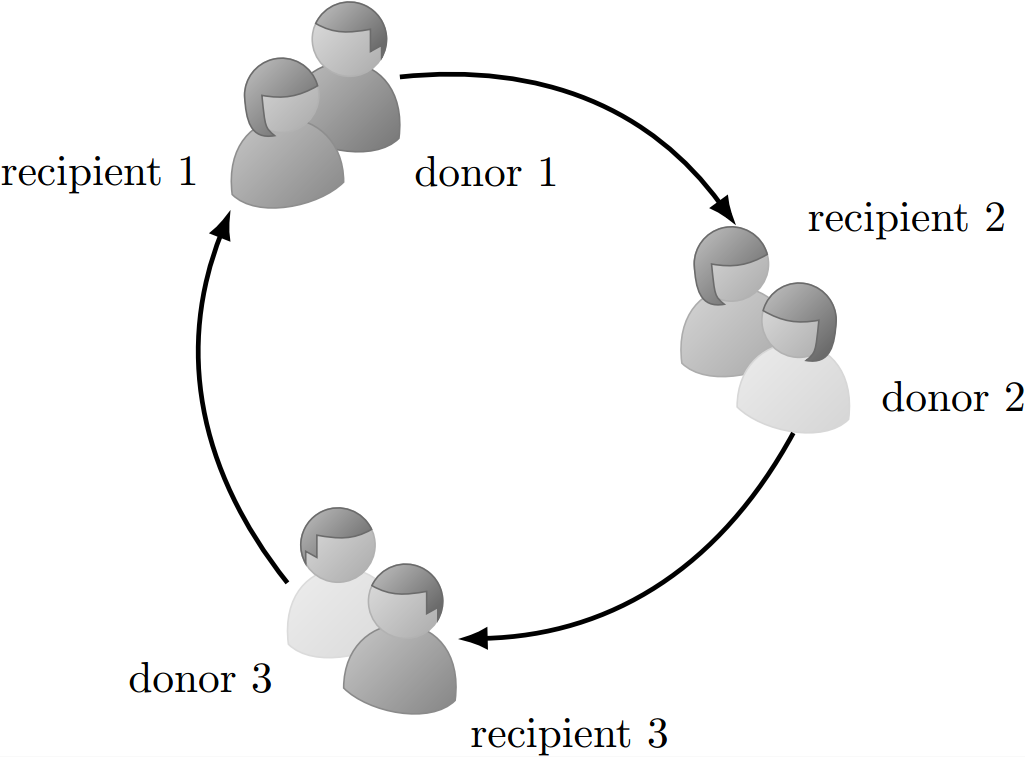
\includegraphics[width=62mm]{../docs/RDP-3pair-cycle} & 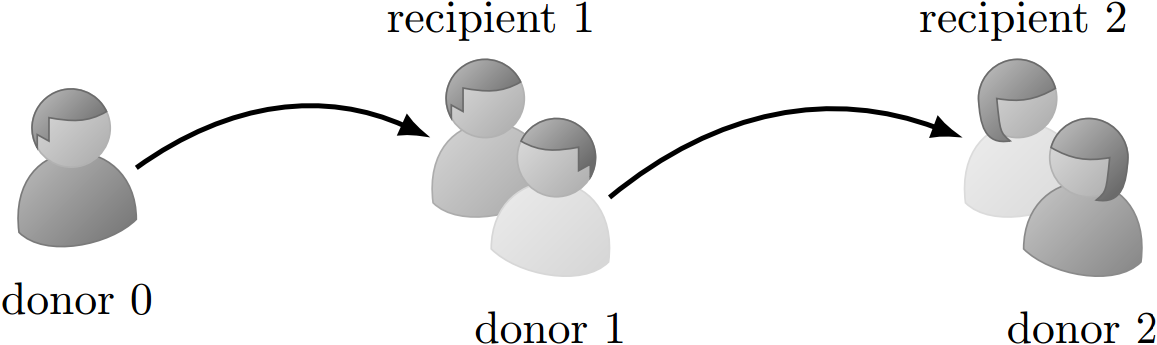
\includegraphics[width=62mm]{../docs/RDP-3pair-chain} \\
\end{tabular}

\subsection{Kezdeti kérdések}
Ahhoz, hogy a projekt használhatósága és a valóságot minél jobban modellező szemlélete megmaradjon \viki[az alábbi kérdéseket, majd válaszokat gyűjtöttem össze]{Egyébként jól értelmezem, hogy ez a Questionary amit kaptunk, az nem publikus? Ha igen, akkor utána fogok kérdezni ennek a hivatkozása hogy történik.}. Ezek segítenek a modell kialakítása során megtalálni a szükséges paramétereket és értékkészletüket.

\emph{Összefoglalás}

\section{Felhasznált adathalmaz}

A kezdeti kérdések alapján körvonalazódott modellezéshez a \href{https://researchdata.gla.ac.uk/1878/}{University of Glasgow vesecsere programok optimalizálásához szintetikusan előállított adathalmazát} használom fel, valamint bővítem ki.
\viki{Ezen most nem látszik a dokumentumban, hogy egy klikkelhető link, illetve ha valaki kinyomtatja (idősebb korosztály szokott ilyet), akkor elveszik az infó.}
\viki{A University of Glasgow-nak szerintem Glasgow-i Egyetem a magyar neve (https://hu.wikipedia.org/wiki/Glasgow-i\_Egyetem).}

\subsection{Adathalmaz jellemzése}

\viki[Tartalmaz egyes szintetikusan generált eseteket]{Ez úgy hangzik, mintha mást is tartalmazna, pedig nem.} és felhasználási módja közé tartozik tesztelni és összehasonlítani különféle vesecsere program optimalizáló technikákat.

180 darab különböző vesecsere probléma esetet tartalmaz JSON formátumban. A JSON fájlok nevei egyben megadják az adott eset paramétereit is.
A nevek eleje egységesen:
uk\_2019\_splitpra\_bandxmatch\_pra0\_pdd,
majd egy alsóvonás jellel elválasztva követi az
<alt>\_<size>-<iteration>.json szöveg.
A relációs jelek közé írt értékek jelentése:
\begin{itemize}
	\item alt - altruista donorok aránya
	
	Értékkészlet: 0.05, 0.10, 0.20

	\item size - recipiensek száma
	
	Értékkészlet: 50, 100, 200, 500, 750, 1000

	\item iteration - különböző véletlenszerű esetek
	
	Értékkészlet: 0-9
\end{itemize}

\subsection{Jelenlegi adatmezők}

\viki{Nagyon zavaróak itt az egész fejezetben a zárójelbe tett angol JSON mező nevek. Megakasztják / döcögőssé teszik az olvasás flowját. Ha valaki pedig valamelyik mező jelentését keresi, akkor ebben az ömlesztett szövegben úgyse fogja megtalálni. Én különválasztanám a mesét, hogy mit tartalmaz az adathalmaz és a JSON adatmezők nevének a jelentését. Ez utóbbit valamilyen szépen formázott módon, pl. táblázattal, vagy egy kis példán keresztül szemléltetve raknám a fejezet végére egy technikaibb szekcióba. \\ Egy profi író mindig figyel az olvasóközönségére is: a te olvasóközönséged két jól elkülönülő táborból áll, VIK-es hallgatókból és SZIT-es matematikusokból. Az utóbbiakat nem fogja érdekelni a JSON definíciója, ha ezt egy skippelhető alfejezetbe szeded ki, az növelni fogja a dolgozatod minőségét és olvashatóságát az ő szemükben.}

Minden JSON-fájl két fő részből áll. A donor-oldal (data) tartalmazza a dage mezőt (donor kora), a bloodtype mezőt (vércsoport: A, B, O vagy AB), az altruistic jelzőt (altruista donor-e), a sources mezőt (a hozzákapcsolt recipiens azonosítója, altruistáknál hiányzik), valamint a matches tömböt, amely az éleket írja le: minden él egy recipiens azonosítóból és egy score értékből áll. Ez utóbbi egy 0--100 közötti, előre aggregált kompatibilitási pontszám, \viki[valószínűleg UKLKSS-alapú HLA-mismatch érték]{Az olvasó ezt nem fogja érteni, el kellene magyarázni mit jelent.}.

A recipiens-oldal (recipients) tartalmazza a cPRA mezőt (\viki[kalkulált PRA-érték, 0 és 1 között]{Én ettől még nem lennék okosabb, hogy ez mit jelent. Ezek a kifejezések (UKLKSS, HLA-mismatch, cPRA, PRA) egyébként mehetnének a Szakkifejezések fejezetbe.}), a bloodtype mezőt, valamint a hasBloodCompatibleDonor jelzőt, amely azt mutatja, van-e vércsoportilag kompatibilis donora az adott recipiensnek.

A jelenlegi solver kizárólag a gráfstruktúrát és az élsúlyokat (score) használja. A cPRA, dage, bloodtype és hasBloodCompatibleDonor mezők a jelenlegi modellben figyelmen kívül maradnak.

\subsection{Hiányzó mezők és lehetséges kiegészítések}

A recipiens kora (rage) hiányzik az adatokból, holott a donor--recipiens korkülönbség fontos minőségi kritérium, és a donor kora (dage) már elérhető. Szintetikus generálással pótolható \viki[UK KEP]{Az olvasó nem tudja, hogy ez mi.} eloszlás alapján.

A várakozási \viki[idő]{typo: időnek} (waiting\_time, napokban) a README szerint szerepelnie kellene, de a tényleges JSON-fájlokból hiányzik. Ez a \viki[Light-Equity optimalizálási policy]{Az olvasó nem tudja, hogy ez mi.} egyik alapja lenne. \viki[UK historikus eloszlásból]{Ez ugyanaz mint a UK KEP eloszlás? Konzisztensen ugyanolyan néven hivatkozz rá.} generálható.

A \viki[highly\_sensitised logikai jelző]{Az olvasó nem tudja, hogy ez mi (itt mondjuk tippelni tud, de le kell írni precízen).} szintén ígérve van a README-ben, de nincs jelen. \viki[Triviálisan]{Ezt a szót érdemes kerülni, sokan (köztük én is) lekezelőnek tartják. Bőven elég azt mondani, hogy levezethető a következőképpen, a levezetés nehézségét nem érdemes minősíteni, mert az szubjektív.} levezethető: cPRA értéke meghaladja-e a 0.85 küszöböt.

Az ország-azonosító (country) nélkülözhetetlen a páneurópai Egyéni Racionalitás elemzéséhez és az együttműködési politikák kiértékeléséhez. Szintetikusan hozzárendelhető, például 5 ország arányos elosztásával.

A távolság (distance\_km) él-szintű mező jelenleg nincs jelen, holott az EURO-KEP főváros-távolságot tervez közelítőként használni. Számítható, ha az ország-azonosító rendelkezésre áll.

\viki[HLA allél adatok (A, B, C, DR, DQ lókuszok)]{Az olvasó nem tudja, hogy ez mit jelent.} nem szerepelnek az adathalmazban, csak az aggregált score érték. Emiatt az \viki[Eurotransplant és a HLA Working Group pontszámok]{Ezekről sem tudjuk mit jelentenek.} nem reprodukálhatók; a score valószínűleg UKLKSS-alapú.

A lemondási valószínűség (cancellation\_prob) él-szintű értékként nem szerepel. \viki[Lemondási politikák]{Ez az angol cancellation policy tükörfordítása? Ki kéne fejteni, hogy mit takar (ki hozza meg a döntést, milyen döntések lehetségesek).} modellezéséhez szükséges lenne, és a cPRA értékéből \viki[élenkénti függvénnyel]{Ez mit jelent? A kör éleinek a cPRA adataiból képzett fv?} közelíthető.

A kompatibilis pár jelző (is\_compatible\_pair) nincs külön tárolva. A kompatibilis pár-politika \viki[(KEP-be lépési döntés minőségi feltétellel)]{Erről kéne többet írni, hogy mit jelent.} szempontjából szükséges; a hasBloodCompatibleDonor mezőből részben következtethető.

Az LKDPI összetevői (magasság, súly, vérnyomás, eGFR, dohányzás) nem elérhetők, csak a donor kora (dage) áll rendelkezésre. A teljes LKDPI-index így nem számítható.

A centrum-azonosító (center\_id) sem szerepel az adatokban, holott a különböző transzplantációs centrumok eltérő kapacitáskorlátokkal rendelkezhetnek. Szintetikusan hozzárendelhető.

\viki{Általános megjegyzés a fenti fejezethez: ezt maximum egy, a témában kifejezetten jártas szakértő fogja megérteni, tele van szakzsargonnal és a zárójeles magyarázatok sem segítenek sokat, esetleg mégtöbb szakzsargont tartalmaznak. Gondolj pl. a kollégiumi szobatársadra és írj úgy, hogy ő is megértse.}

\subsection{Amit a solver már most felhasználhatna}

\viki{Ezt a fejezetet nem teljesen értem, amiket itt írsz az előző fejezetben is szerepeltek. Az előző fejezetben lévő és itt nem megemlített dolgokat nem tudná felhasználni a solver?}

A cPRA értéke alapján az erősen érzékenyített recipiensek (cPRA nagyobb mint 0.85) preferálhatók lennének az \viki[objektívfüggvényben]{Magyarul célfüggvény.}, például egy \viki[bónusztaggal]{Ez a bónusz szó furcsa. Szorzóval? Illetve a szorzatnak tényezői vannak, az összegnek vannak tagjai.} súlyozva az élsúlyt.

Ha a recipiens kora (rage) is megvolna, a donor--recipiens korkülönbség beépíthető lenne élsúlyként.

A hasBloodCompatibleDonor jelző alapján a kompatibilis párok azonosíthatók, és más belépési feltételekkel kezelhetők: csak akkor lépnek be a KEP-be, ha a csere minőségi javulást hoz, és legfeljebb 1--3 futtatáson maradnak.

A cPRA-ból per-él lemondási valószínűség számítható. Ekkor az objektív nem a nyers score-t, hanem a várható értéket maximalizálja, azaz a score és az 1 mínusz a lemondási valószínűség szorzatát.

\begin{figure}[htbp]
  \centering
  \begin{subfigure}[b]{0.42\textwidth}
    \centering
    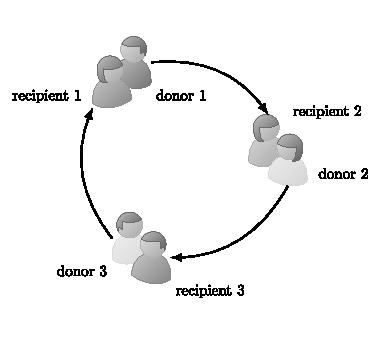
\includegraphics[width=\linewidth]{Figures/cycle}
    \caption{Example of a cycle~\cite[Figure~1]{barkel2026}.}
  \end{subfigure}
  \hfill
  \begin{subfigure}[b]{0.54\textwidth}
    \centering
    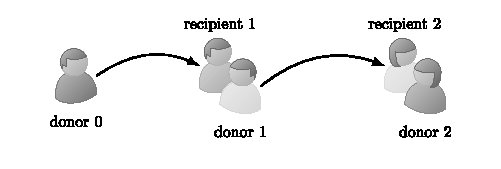
\includegraphics[width=\linewidth]{Figures/chain}
    \caption{Example of a chain~\cite[Figure~2]{barkel2026}.}
  \end{subfigure}
\end{figure}

\bibliographystyle{abbrvnat}
\bibliography{X6E3NN}

\end{document}
